\documentclass[border={0pt -30pt 0pt -15pt}]{standalone}
\usepackage{pgfplots}
\usepackage{tikz}

\begin{document}
  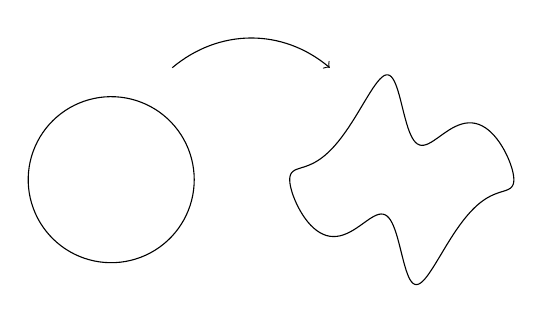
\begin{tikzpicture}
    \begin{axis}[axis lines=none, axis equal,
      xmin=-3,xmax=10
      % grid=both,
      ]
      \addplot [domain=0:360,samples=100]({2*cos(x)},{2*sin(x)});
      \addplot[domain=0:360,samples=200]({7 +
        (1-cos(x*2)/2)*1.8*sin(x)},{(1-sin(x*4)/2)*1.8*cos(x)});
      \node[anchor=west] (source) at (axis cs:1.0,2.5){}; \node
      (destination) at (axis cs:5.5,2.5){}; \draw[->](source) to
      [out=40,in=140] (destination);
    \end{axis}
  \end{tikzpicture}
\end{document}